\section{Experimental Evaluation}
\label{sec:eval}
% Validate the claims that you have done in 3. and introduction.

% Here you think what you need to demonstrate and how to best demonstrate it
% (what kind of graphs, tables, etc are needed). You can do the experimental evaluation
% (i.e., running/benchmarking the futhark programs and gathering performance data)
% at this point, once you put some though into what this should be.

% - The full brute force
% - Implementation with slow brute force
% - Implementation with fast brute force
% - Implementation with fast brute force and merge sort
% - Implementation with fast brute force and radix sort
% - Implementation with fast brute force, radix sort and partition
% - Implementation with fast brute force, radix sort, partition and fixed traversal
% - Implementation with fast brute force, radix sort and leaf sort
% - Implementation with fast brute force, radix sort, leaf sort and fixed traversal


This section describes and demonstrates the performance of each optimisation described in sections \ref{sec:kdtree} and \ref{sec:traversal}, as well as the overall performance gains achieved of the k-d tree solution compared to the brute force from section \ref{sec:brute}.
\\[2mm]
Each solution has been validated against the result of the brute force solution, using Futhark benching.  


\subsection{Optimisation using Sorting over Partition}

The following subsection demonstrates the results for solutions using partition and sorting, respectively, described in section \ref{sec:kdtree}. 


\begin{figure}[H]
\centering
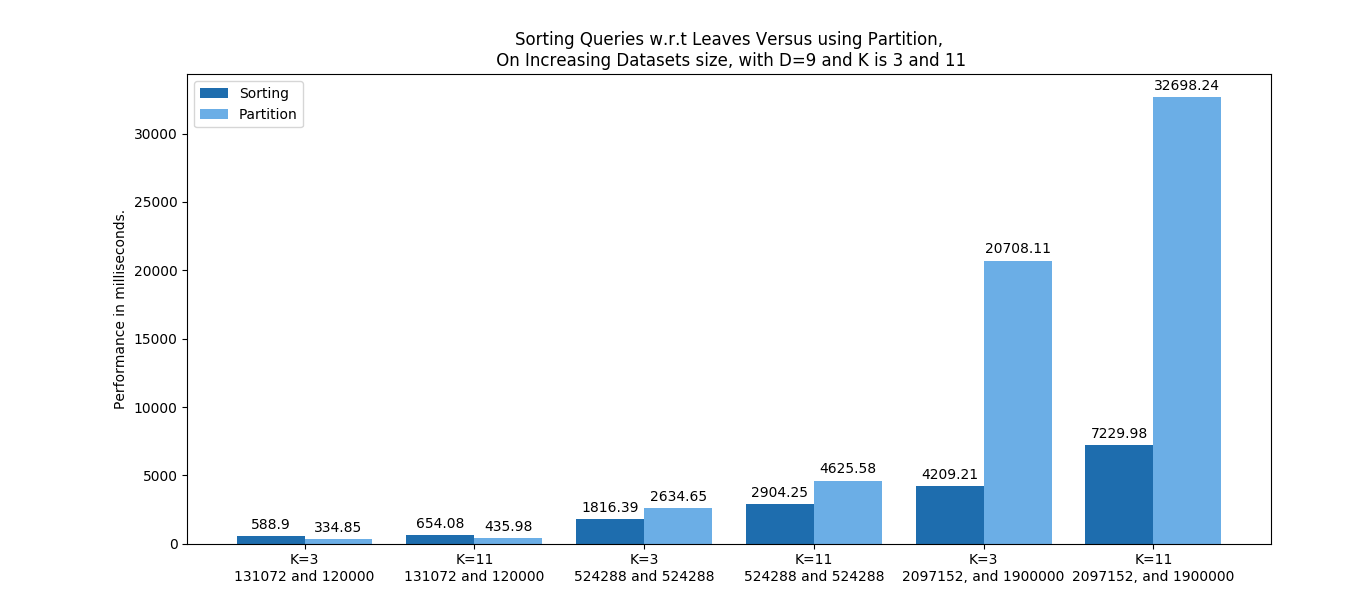
\includegraphics[width=1\textwidth]{pics/plot-figs/new-sort-all-d9.png}
\caption{Testing for D=9 with datasets of sizes‚ 2097152 and 1900000, 524288 and 524288, and 131072 and 120000.}
\label{fig:sort1}
\end{figure}

In figures \ref{fig:sort1} and \ref{fig:sort2}, we compare the performances between sorting and partition. It shows that sorting works faster for datasets larger than 524288, with higher dimensionality such as D=9, or lower dimensionality such as D=4 with a high K, such as K=11. 

\begin{figure}[H]
\centering
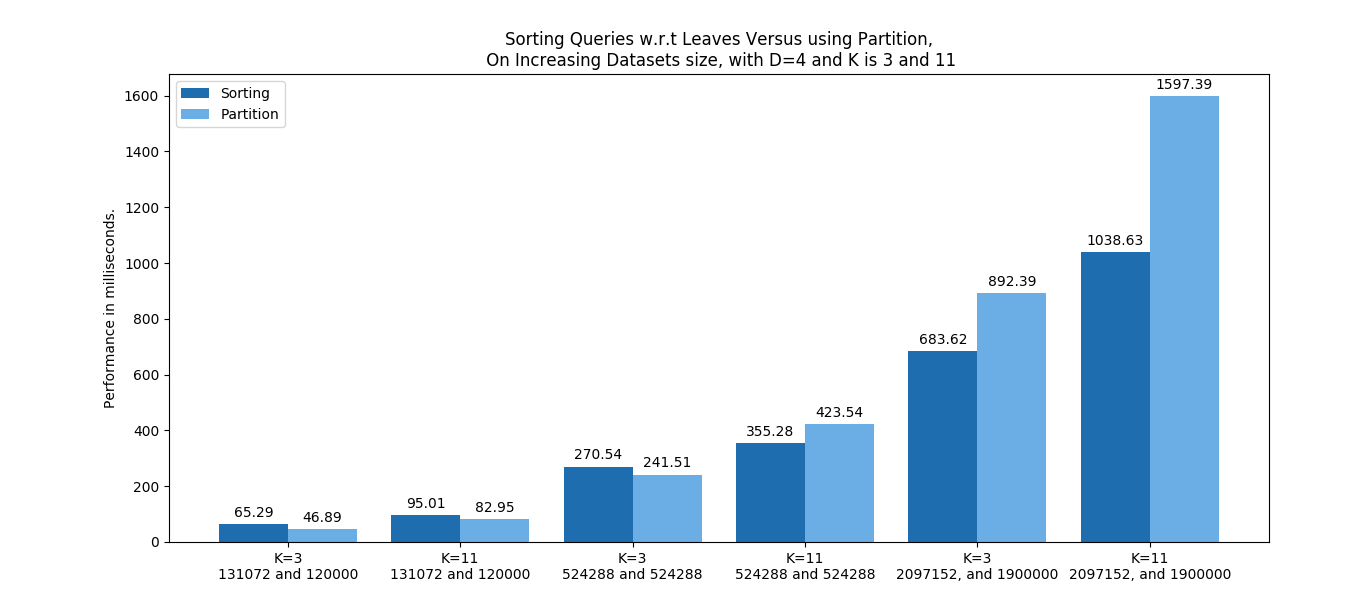
\includegraphics[width=1\textwidth]{pics/plot-figs/new-sort-alld4.png}
\caption{Testing for D=4 with datasets of sizes‚ 2097152 and 1900000, 524288 and 524288, and 131072 and 120000.}
\label{fig:sort2}
\end{figure}



% Speedups: 
% D=9 [0.56, 0.66, 1.45, 1.59, 4.91, 4.52]
% D=4 [0.71, 0.87, 0.89, 1.19, 1.3, 1.53]

% \begin{figure}[H]
%   \centering
%   \subfloat[D=16, K=3 and K=11.]{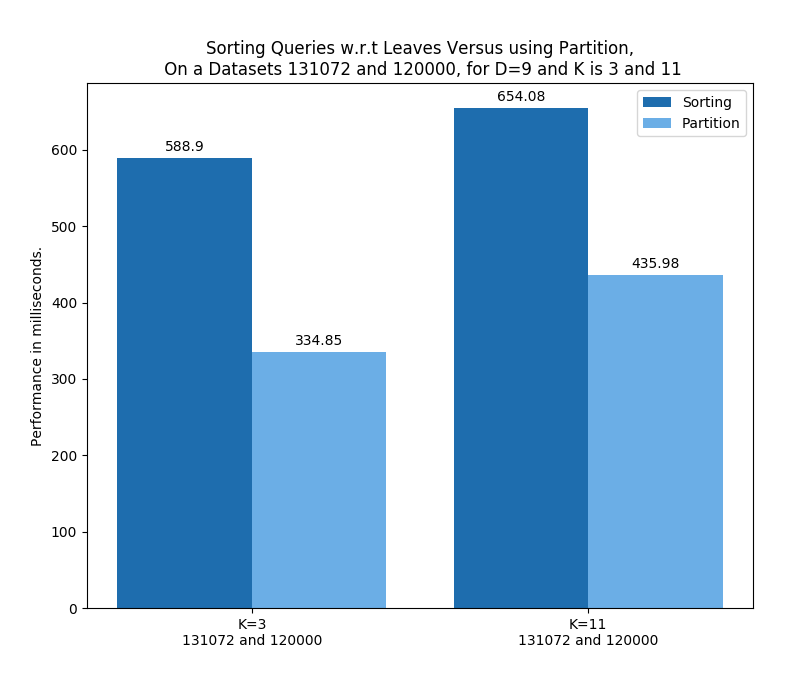
\includegraphics[width=0.49\textwidth]{pics/plot-figs/new-sort-d9-k3k11.png}\label{fig:f1}}
%   % \hfill
%   % \hspace{0.cm}
%   \subfloat[D=4, K=3 and K=11.]{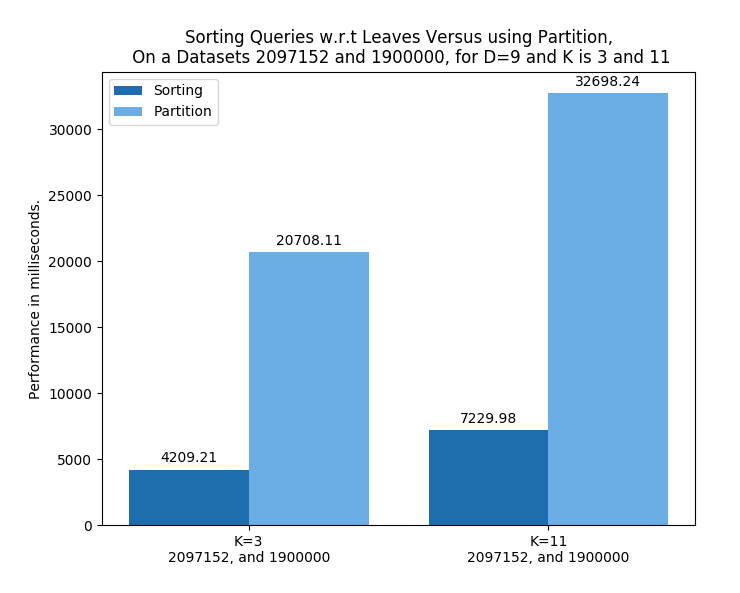
\includegraphics[width=0.5\textwidth]{pics/plot-figs/new-sort-d9-k3k11-big.png}\label{fig:f2}}
%   \caption{Dark blue representing sorting queries and light blue representing using partition, on datasets of sizes 2097152 and 1900000, and 131072 and 120000.}
% \label{fig:sort1}
% \end{figure}

However, by looking at the speed-ups presented in table \ref{tab:sort}, we see that K does not have any remarkable effect, since the speed-up is higher for K=3 on the dataset of size 524288, and the speed-up is higher for K=11 on the dataset of size 2097152. We also see that increasing D has a positive effect on the speed-ups. The datasets of sizes 2097152 and 1900000 have a speed-ups that are 3.61 and 3.99 times higher when using a dimension of size 9 over 4. 

\begin{table}[H]
\centering
\begin{tabular}{@{} *8l @{}}    \toprule
\emph{D} & \emph{K=3} & \emph{K=11} & \emph{K=3} & \emph{K=11} & \emph{K=3} & \emph{K=11} &  \\\midrule
  4  & 0.71 & 0.87 & 0.89 & 1.19 & 1.3 &1.53  &   \\ 
  9  & 0.56 & 0.66 & 1.45 & 1.59 & 4.91 & 4.52  &   \\\bottomrule 
 \hline
\end{tabular}
\caption{Speed-ups gained by increasing the dataset sizes, for sorting against partition.}
\label{tab:sort}
\end{table}
 

%  achieve a speed-up of almost $13$, whereas with D=4 and K=11 we achieve a speed-up of almost $2$, and while the latter is still a considerable speed-up, it is clear that high dimensionality and a large K is where the sorting solution excels, as it shows in the former speed-up. However, these tests are made on large dataset sizes of 2097152 and 1900000, and if we try to do the same test on smaller datasets of sizes 131072 and 120000, it shows that the solution using partition outperforms the sorting solution with a factor of $1.2$. 
% However, this refers to figure \ref{fig:f4}, with D=4, whereas figure \ref{fig:f3}, with D=16 shows that the sorting solution still outperforms the partition solution with a factor of $3.3$.


% In figure \ref{fig:sort1}, we look to compare the performances between sorting and partition. For a D=9, we achieve a speed-up of almost $13$, whereas with D=4 and K=11 we achieve a speed-up of almost $2$, and while the latter is still a considerable speed-up, it is clear that high dimensionality and a large K is where the sorting solution excels, as it shows in the former speed-up. However, these tests are made on large dataset sizes of 2097152 and 1900000, and if we try to do the same test on smaller datasets of sizes 131072 and 120000, it shows that the solution using partition outperforms the sorting solution with a factor of $1.2$. 
% However, this refers to figure \ref{fig:f4}, with D=4, whereas figure \ref{fig:f3}, with D=16 shows that the sorting solution still outperforms the partition solution with a factor of $3.3$.

% 5866/1754 = 3,3443557583
% 94.64/77.09 = 1,2276559865


% 1487264/117716 = 12,6343402766
% 1814/1114 = 1,6283662478


% \begin{figure}[H]
% \centering
% 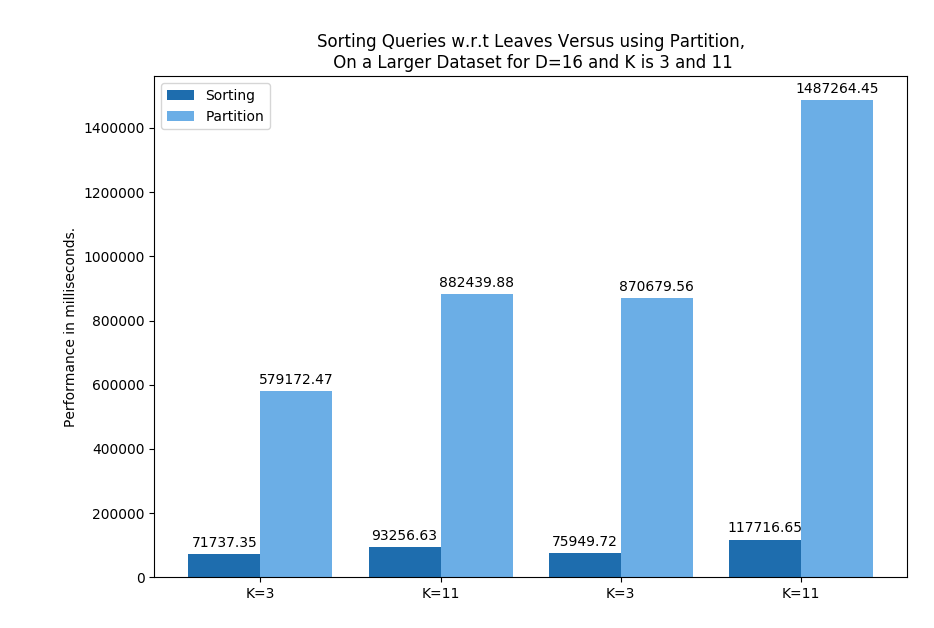
\includegraphics[width=1\textwidth]{pics/plot-figs/sort-d16.png}
% \caption{}
% \end{figure}

% \begin{figure}[H]
%   \centering
%   \subfloat[D=16, K=3 and K=11.]{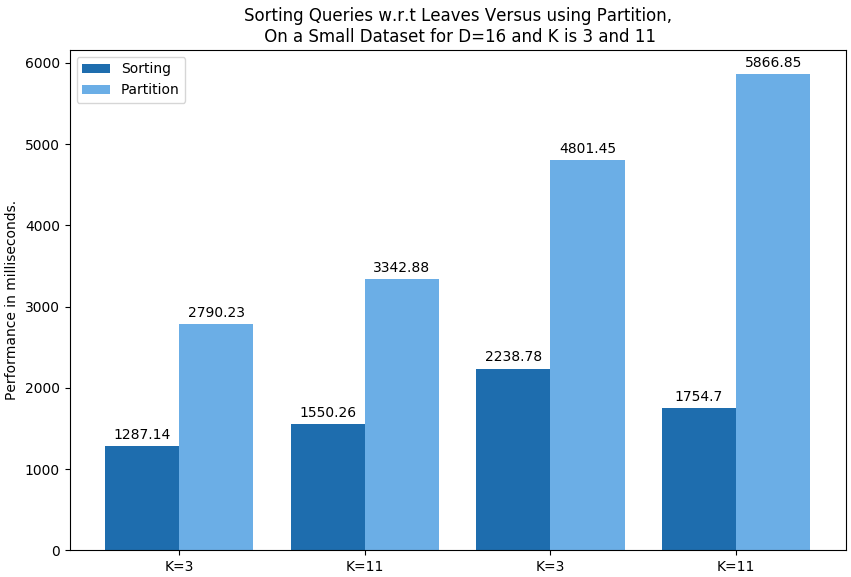
\includegraphics[width=0.49\textwidth]{pics/plot-figs/sort-small-d16.png}\label{fig:f3}}
%   % \hfill
%   % \hspace{0.cm}
%   \subfloat[D=4, K=3 and K=11.]{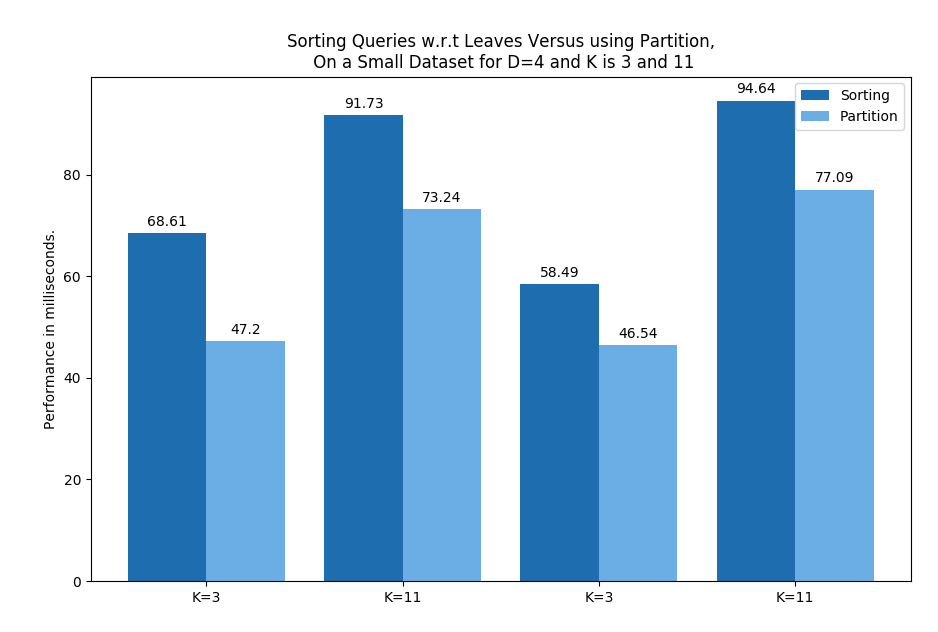
\includegraphics[width=0.5\textwidth]{pics/plot-figs/sort-small-d4.png}\label{fig:f4}}
%   \caption{Dark blue representing sorting queries and light blue representing using partition, on small datasets of sizes 131072 and 120000.}
% \label{fig:sort2}
% \end{figure}

% The previous results cause for curiosity as to which area the ’breaking point’ between using sorting over partition would be. Figure \ref{fig:sort3} tests on a small K=3 and small datasets of sizes 131072 and 120000, in which the D is increasing in size. Here we see that for this example, D would have to be at least 13 for sorting to outperform partition.


% \begin{figure}[H]
% \centering
% 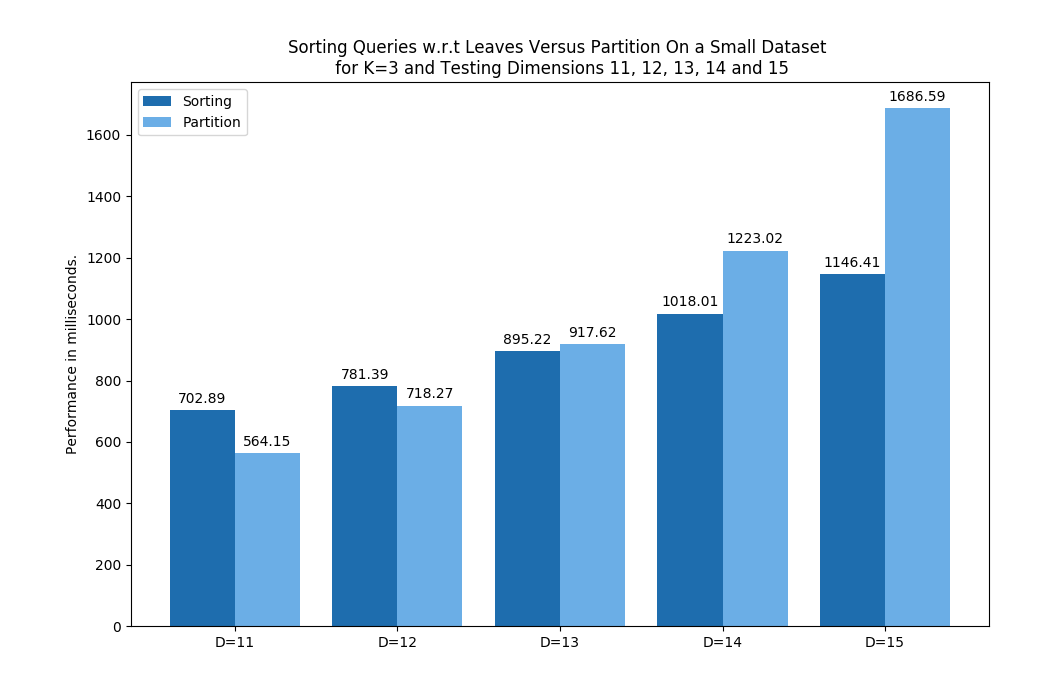
\includegraphics[width=1\textwidth]{pics/plot-figs/sort-mult-d-big.png}
% \caption{Finding the 'breaking point' of D in which the sorting solution becomes faster, for K=3 and datasets of sizes 120000 and 131072.}
% \label{fig:sort3}
% \end{figure}


In conclusion, we see that sorting works incrementally better for increasing sizes in D and datasets. 


\subsection{Optimising Tree Traversal with Full Dimensionality Checking}
\label{sec:evaltrav}

The following demonstrates the results for the optimisation described in section \ref{sec:traversal}. 


\begin{figure}[H]
\centering
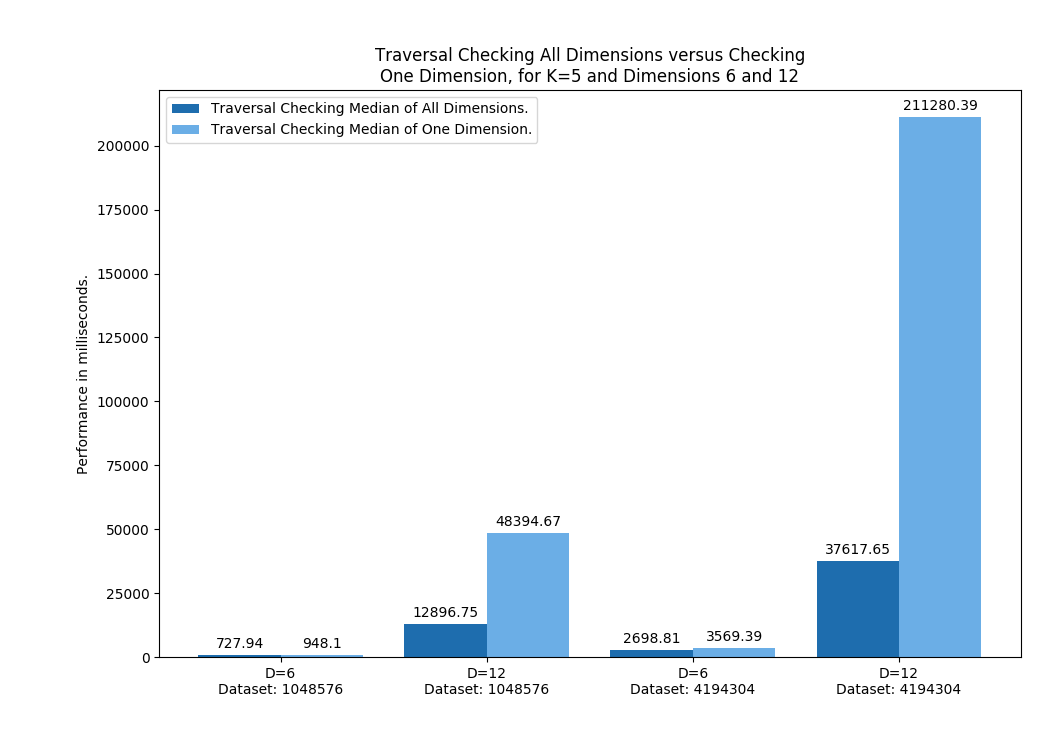
\includegraphics[width=1\textwidth]{pics/plot-figs/new-trav-k5-d6d12.png}
\caption{Traversal comparing results w.r.t varying sizes for D on a smaller and larger dataset.}
\label{fig:trav1}
% \caption{The HDF5 hierarchical and cyclic grouping options \protect\cite{hdf5}.}
\end{figure}

Figure \ref{fig:trav1} shows that increasing the size of D as well as the dataset sizes will give a better performance for the optimised solution that checks at all dimensions. The test uses a static size K=5 and tests on D=6 and D=12 for both small and large datasets, where the light blue is the traversal checking one dimension and the dark blue is the traversal checking all dimensions. In comparison, the speed-ups for D=12 is 2.45 and 4.3 times faster than D=6, respectively. 

% \todo[color=green!40, inline, size=\small]{Beskriv tarverse ift. K}
% [1.3024425089979943, 3.752470195979607, 1.322579210837369, 5.616522829044345]

% [2.47, 4.47, 4.3, 3.14, 3.37, 2.65]
\begin{table}[H]
\centering
\begin{tabular}{@{} *5l @{}}    \toprule
\emph{Datasize} & \emph{K=1} & \emph{K=5} & \emph{K=17} &  \\\midrule
Small     & $2.47$  & $4.47$  & $4.3$  &   \\ 
Large     & $3.14$ & $3.37$ & $2.65$ & \\ \bottomrule
 \hline
\end{tabular}
\caption{Speed-ups gained by increasing the size of K for both small and large datasets.}
\label{tab:travk}
\end{table}

\todo[color=green!40, inline, size=\small]{Ret med friske øjne}

The next illustration, figure \ref{fig:trav2}, we analyse whether increasing or decreasing K amounts to a speed-up. Testing against a D=12 for both small and large datasets the speed-ups visible in table \ref{tab:travk} show that the performance in both cases are best with a K=5, however, it shows no correlation between a small or large K amounting 

and more so for larger datasets--which mores visible in table \ref{tab:travk}, which shows the actual speed-ups from the graph in figure \ref{fig:trav2}.

% 8563/3882 = 2,2058217414
% 13082/5946 = 2,2001345442
% 22904/9783 = 2,3412041296

% 30748/10677  = 2,8798351597
% 58172/19044  = 3,054610376
% 111723/36649 = 3,0484597124


\begin{figure}[H]
\centering
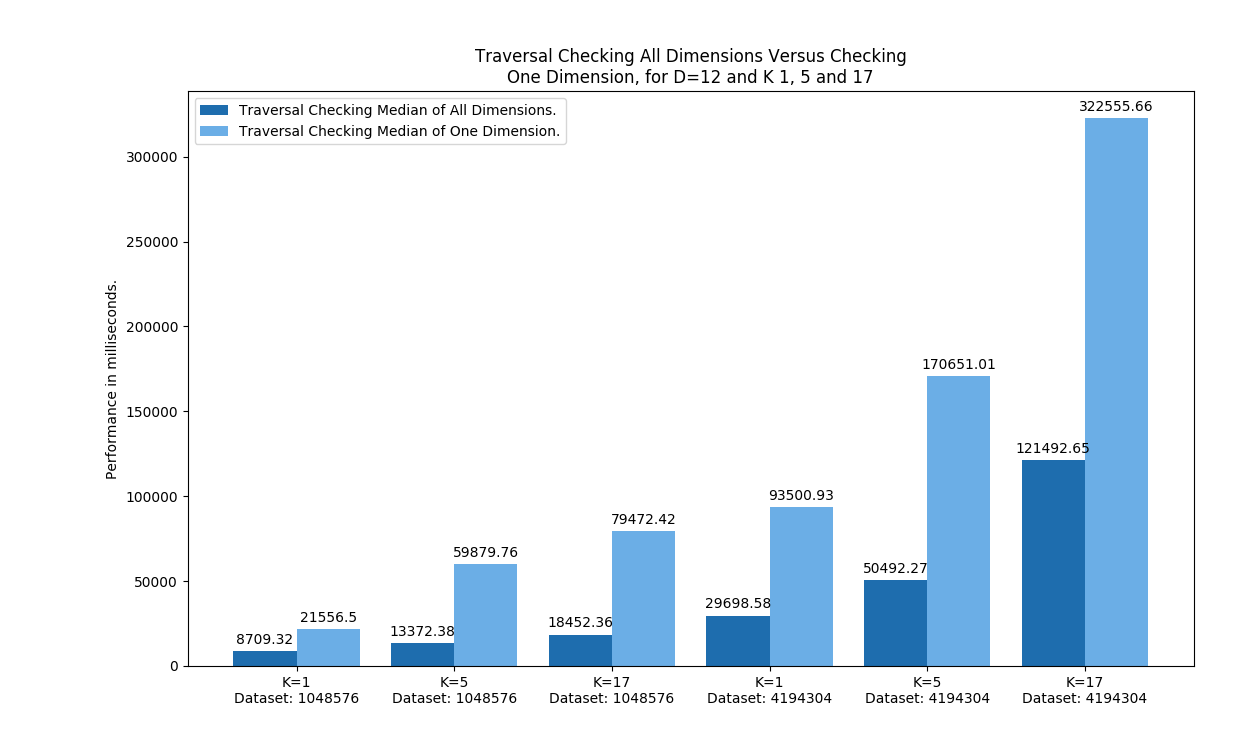
\includegraphics[width=1\textwidth]{pics/plot-figs/new-trav-d12-k1k5k17.png}
\caption{Traversal comparing results w.r.t varying sizes for K on a smaller and larger dataset.}
\label{fig:trav2}
\end{figure}


\subsubsection{Demonstrating a Comparison of the Number of Leaf Visits}
\label{sec:evaltravhist}

The following histograms demonstrate the number of visits to leaves performed when searching for the exact KNN. The size of the visits-array is initialised to the total number of leaves,  after which each search iteration will store the number of new visits in the array. The small example below shows that the program would finish finding the exact KNN after six iterations of searches through leaves. The three -1’s indicating that no further leaves are visited. 
% The first visit is typically close to the total of queries because each query will initially have a leaf to search in, of which it naturally belongs. The consecutive number of visits are on the number of additional leaves being visited in order to achieve the exact KNN. 
$$[100, 99, 85, 62, 33, 18, -1, -1, -1]$$
Thus, in the histograms below, a large number of -1's to the left will indicate a few visits, resulting in better performance, while a large number to the right will indicate many visits and poor performance.  

% The following histograms demonstrate the number of visits to leaves performed when searching for the exact KNN. The visits array is initialised with -1's to the size of the number of leaves. The first visit is typically close to the total of queries because each query will initially have a leaf to search in, of which it naturally belongs. The consecutive number of visits are on the number of additional leaves being visited in order to achieve the exact KNN. 


\begin{figure}[H]
  \centering
  \subfloat[Checking all dimensions.]{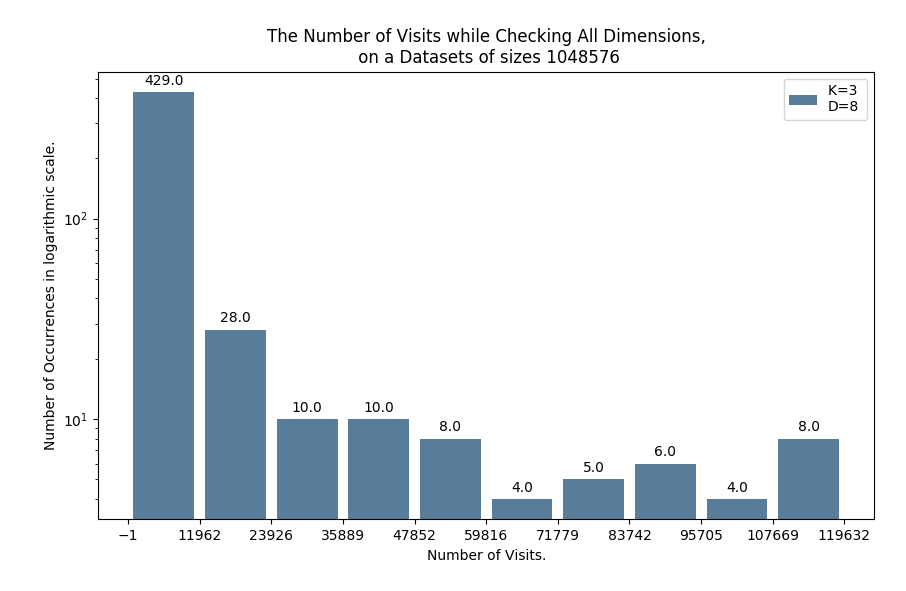
\includegraphics[width=0.49\textwidth]{pics/plot-figs/visits/visit-k3-d8-all-new.png}\label{fig:f5}}
  \subfloat[Checking one dimension.]{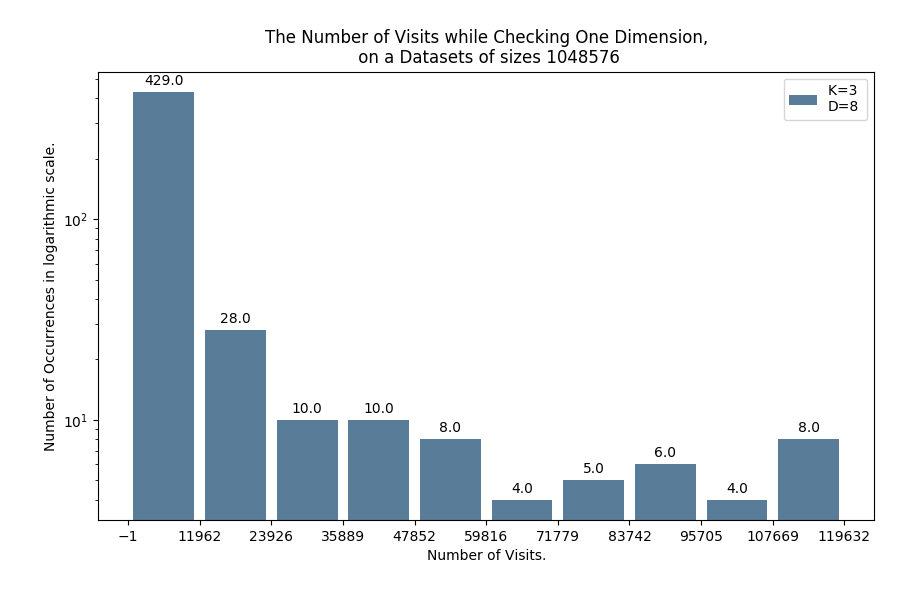
\includegraphics[width=0.5\textwidth]{pics/plot-figs/visits/visit-k3-d8-one-new.png}\label{fig:f6}}
  \caption{Figure a and b show the same result for K=3 and D=8 on both traversal solutions, on datasets of sizes 1048576.}
  \label{fig:k3d8}
\end{figure}


As figures, \ref{fig:f5} and \ref{fig:f6}  demonstrate, for a small K of size 3 and a relatively small D of size 8, we see that the number of visits to leaves in both solutions is equal. However, figures \ref{fig:f7} and \ref{fig:f8}  show increasing D to 16 drastically changes the outcome, such that the method of checking all dimensions excels. 

\begin{figure}[H]
  \centering
  \subfloat[Checking all dimensions.]{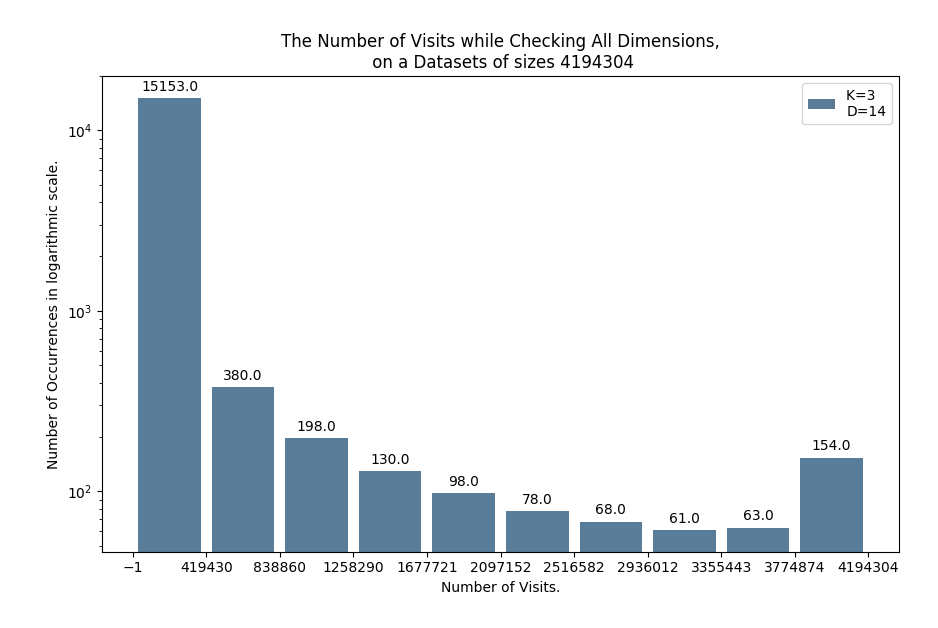
\includegraphics[width=0.5\textwidth]{pics/plot-figs/visits/new-visit-all-k3-d14.png}\label{fig:f7}}
  \subfloat[Checking one dimension.]{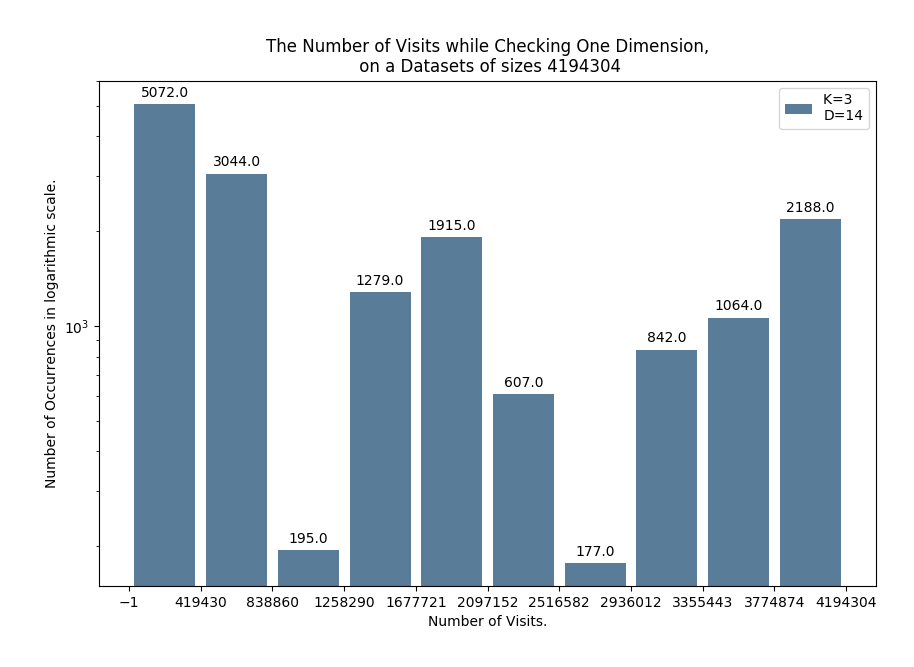
\includegraphics[width=0.5\textwidth]{pics/plot-figs/visits/new-visit-one-k3-d14.png}\label{fig:f8}}
  \caption{Figure a and b show the same result for K=3 and D=14 on both traversal solutions, on datasets of sizes 4194304.}
  \label{fig:k3d16}
\end{figure}


If we experiment further by increasing K to 5 while testing against both a small and large size D, namely 6 and 14, we see in figure \ref{fig:k5d6} that even for a small D there is a slight decrease in the number of visits when checking all dimensions in \ref{fig:f9} compared to checking one dimension in \ref{fig:f10}. The figures in \ref{fig:k5d16} show that for a K=5 and a D=14, the difference is incredibly in favour of the solution checking all dimensions. Thus, all histograms show increasing sizes for K and D will likewise have increasingly better performance on the solution checking all dimensions compared to checking one dimension. 

\begin{figure}[H]
  \centering
  \subfloat[Checking all dimensions.]{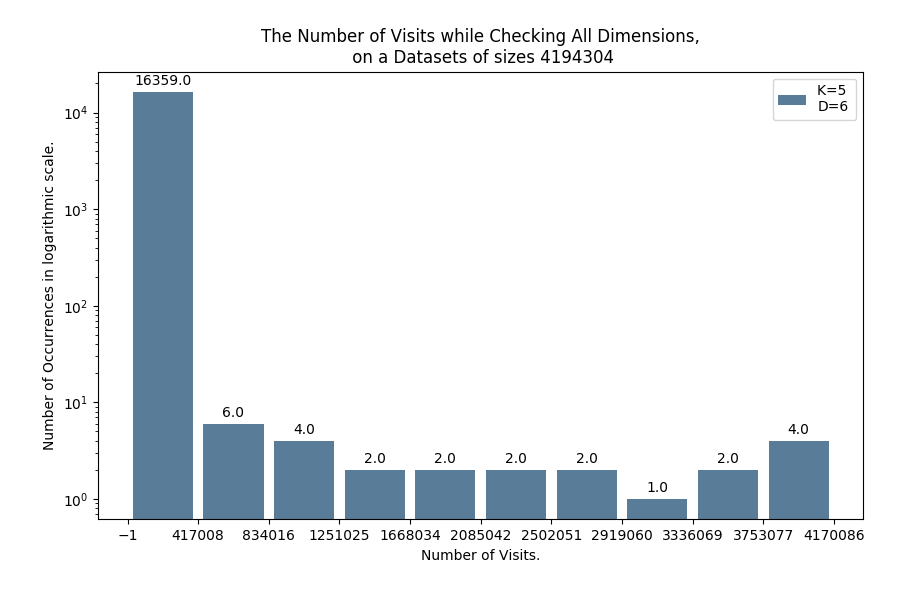
\includegraphics[width=0.5\textwidth]{pics/plot-figs/visits/visit-k5-d6-all-new.png}\label{fig:f9}}
  \subfloat[Checking one dimension.]{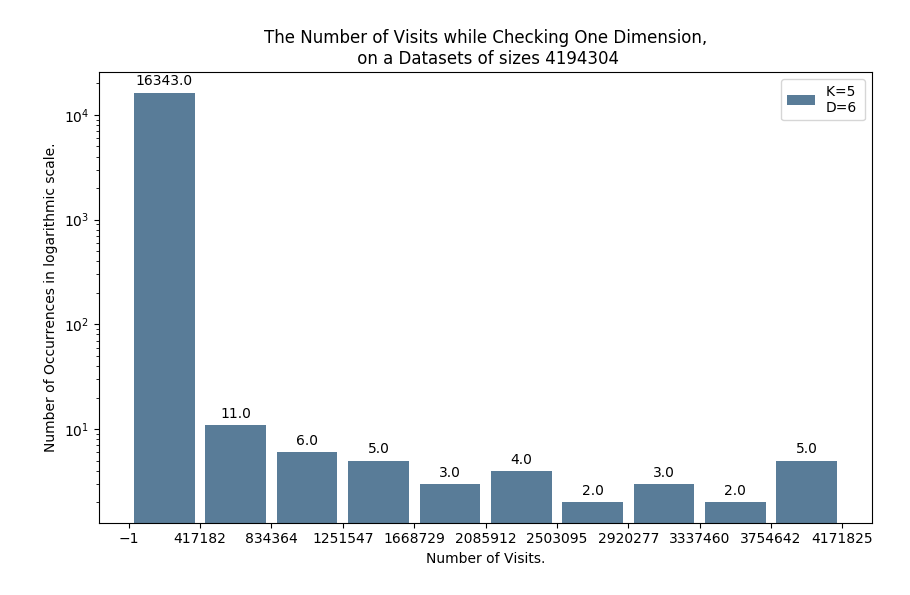
\includegraphics[width=0.5\textwidth]{pics/plot-figs/visits/visit-k5-d6-one-new.png}\label{fig:f10}}
  \caption{Figure a and b show the same result for K=5 and D=6 on both traversal solutions, on datasets of sizes 4194304.}
  \label{fig:k5d6}
\end{figure}


\begin{figure}[H]
  \centering
  \subfloat[Checking all dimensions.]{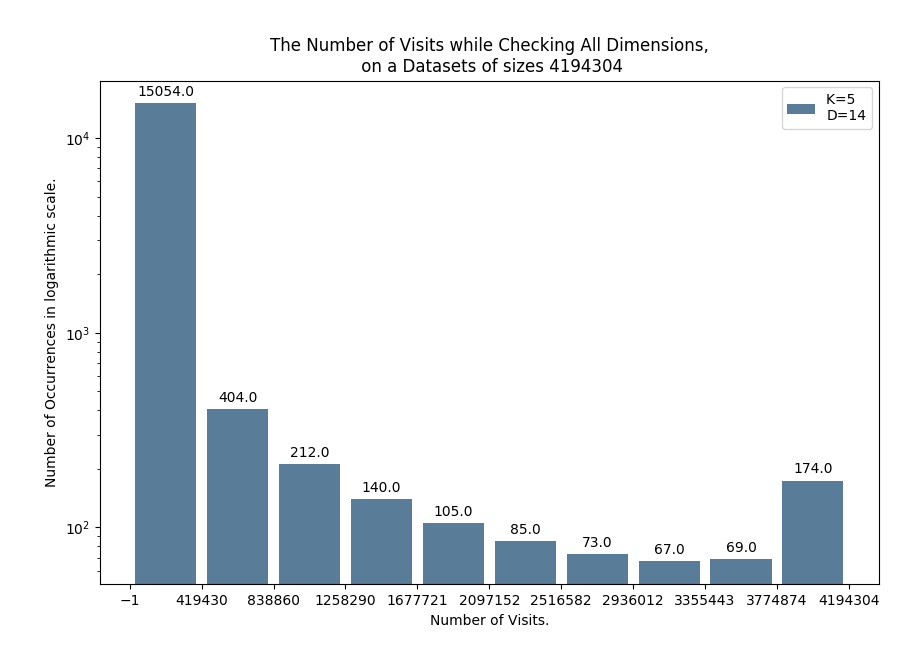
\includegraphics[width=0.5\textwidth]{pics/plot-figs/visits/new-visit-k5-d14.png}\label{fig:f11}}
  \subfloat[Checking one dimension.]{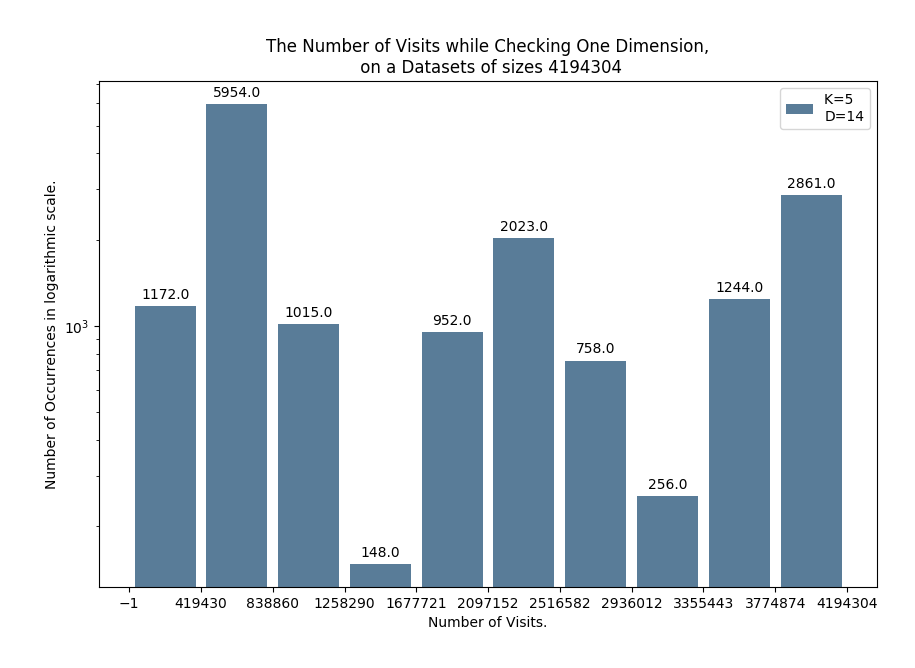
\includegraphics[width=0.5\textwidth]{pics/plot-figs/visits/new-visit-one-k5-d14.png}\label{fig:f12}}
  \caption{Figure a and b show the same result for K=5 and D=14 on both traversal solutions, on datasets of sizes 4194304.}
  \label{fig:k5d16}
\end{figure}




\subsection{Brute Force versus k-d Trees for Computing KNN}



% \begin{figure}[H]
% \centering
% 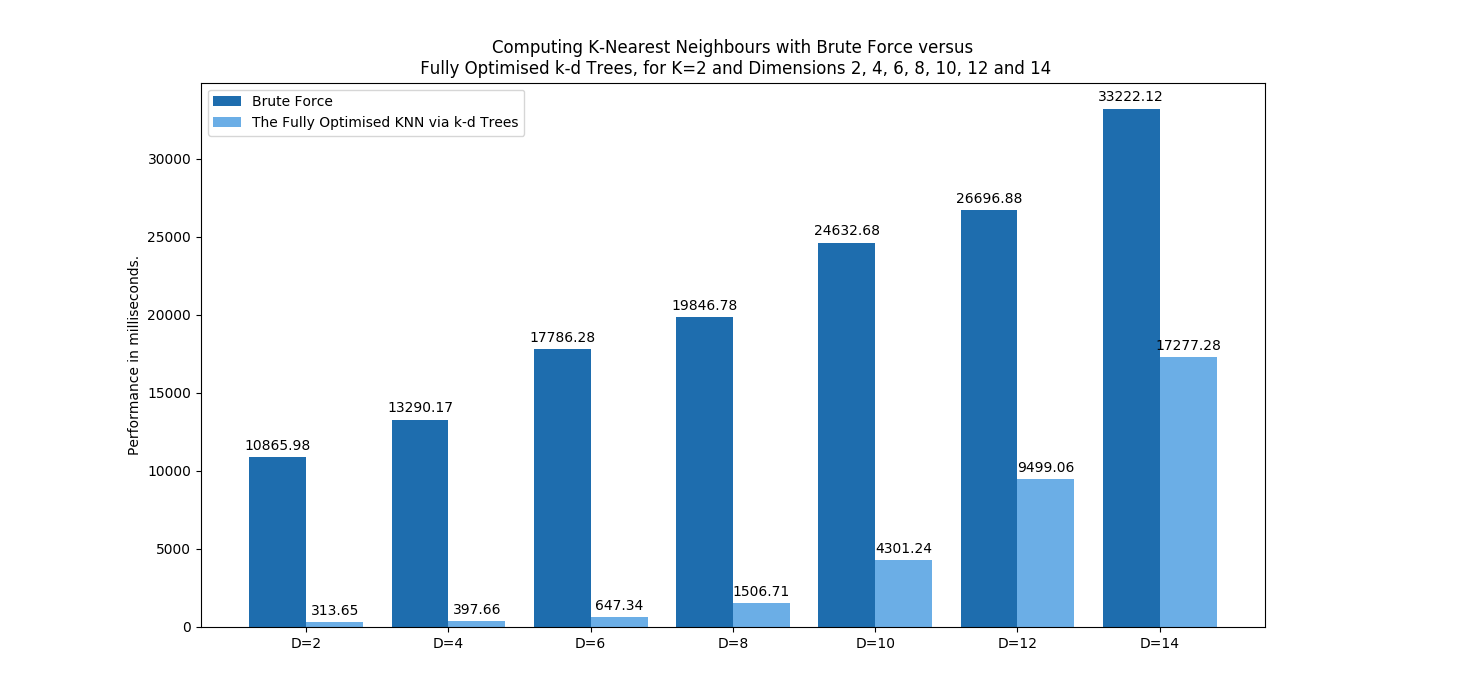
\includegraphics[width=1\textwidth]{pics/plot-figs/brute-mult-k2.png}
% \caption{}
% \label{fig:b1}
% \end{figure}


% \begin{figure}[H]
% \centering
% 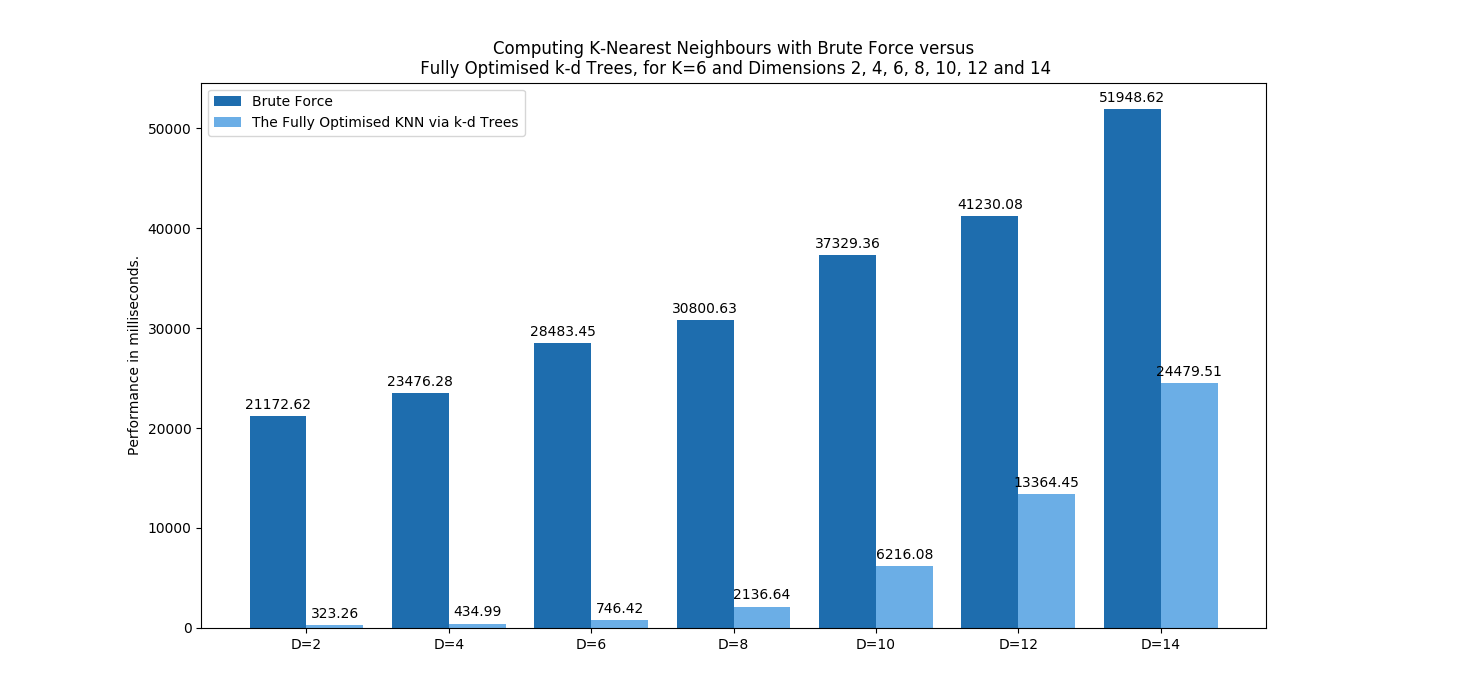
\includegraphics[width=1\textwidth]{pics/plot-figs/brute-mult-k6.png}
% \caption{}
% \label{fig:b2}
% \end{figure}


% \begin{figure}[H]
% \centering
% 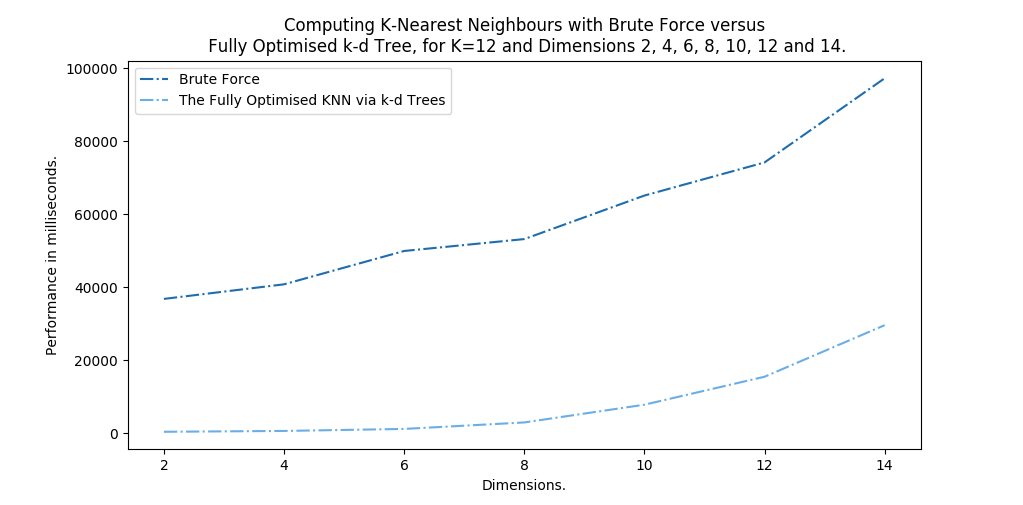
\includegraphics[width=0.8\textwidth]{pics/plot-figs/brute-vs-kdtree.png}
% \caption{}
% \label{fig:b4}
% \end{figure}



% The speed-ups presented in figures \ref{fig:b1}, \ref{fig:b2}, \ref{fig:b3} and \ref{fig:b4} are computed and summarised the the following table \ref{tab:total}. 
% The speed-ups presented in figures \ref{fig:b1}, \ref{fig:b2}, \ref{fig:b3} and \ref{fig:b4} are computed and summarised the the following table 

Table \ref{tab:total} summarises the speed-ups for testing the fully optimised k-d tree implementation against the brute force implementation, where we look at D sizes ranging from 2-14 and K sizes 2, 6 and 12. Figures showing the performance for K=2 and K=6, referenced in the table, can be found in the Appendix \ref{sec:appendix} figures \ref{fig:b1}, \ref{fig:b2} and \ref{fig:b4}.
\begin{table}[H]
\centering
\begin{tabular}{@{} *8l @{}}    \toprule
\emph{K} & \emph{D=2} & \emph{D=4} & \emph{D=6} & \emph{D=8} & \emph{D=10} & \emph{D=12} & \\\midrule
12 & 78.7 & 58.57 & 40.04 & 17.6 & 8.26 & 4.77     &   \\ 
6 & 65.49 & 53.96 & 38.16 & 14.41 & 6.0 & 3.08      & \\ 
2 &  34.64 & 33.42 & 27.47 & 13.17 & 5.72 & 2.81	& \\ \bottomrule
 \hline
\end{tabular}
\caption{Speed-ups achieved by the k-d tree solution compared to the brute force solution, based on datasets of sizes 1048576.}
\label{tab:total}
\end{table}

% [78.7, 58.57, 40.04, 17.6, 8.26, 4.77, 3.27]
% [65.49, 53.96, 38.16, 14.41, 6.0, 3.08, 2.12]
% [34.64, 33.42, 27.47, 13.17, 5.72, 2.81, 1.92]

The results show that any given size of K and D results in a speed-up in favour of the k-d tree solution. This increased performance applies particularly for small dimensions and large K, for instance, K=12 and D=2 result in a speed-up of almost 79. Figure \ref{fig:b3} below illustrates the performance for a static K=12.


\begin{figure}[H]
\centering
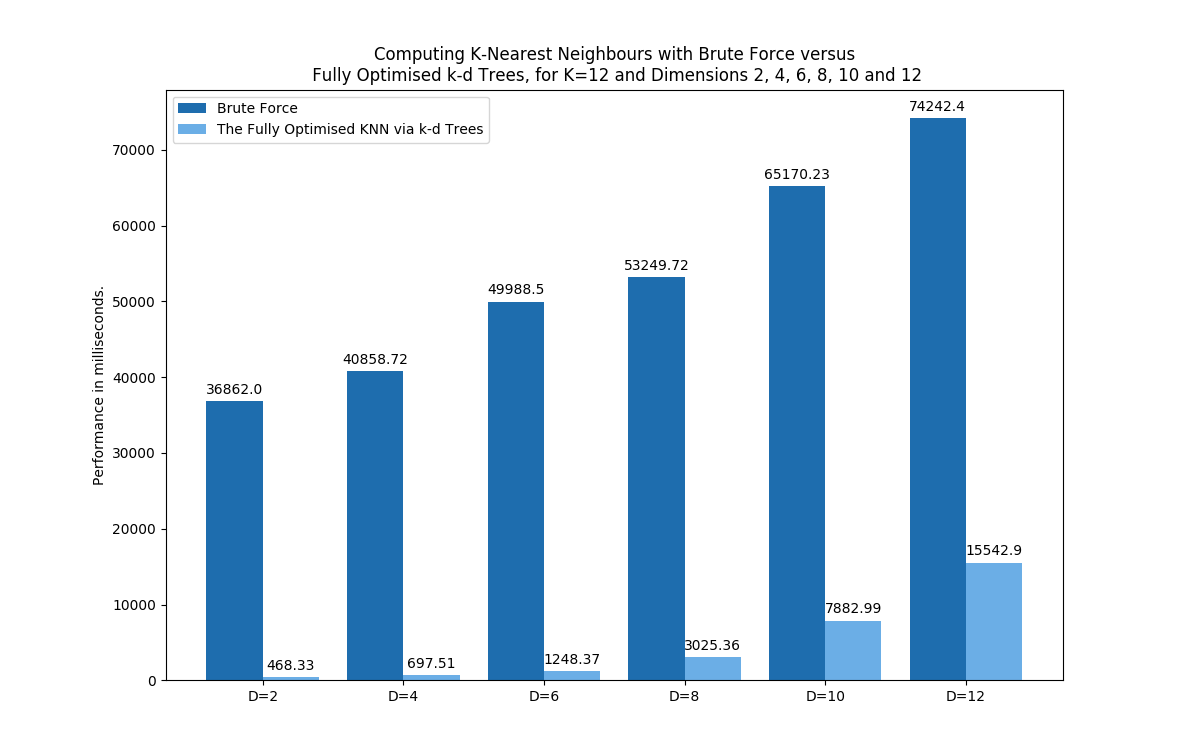
\includegraphics[width=1.1\textwidth]{pics/plot-figs/new-brute-k12.png}
\caption{Performance comparison of k-d tree versus brute force, with a static K=12 on datasets of sizes 1048576.}
\label{fig:b3}
\end{figure}



\begin{figure}[H]
\centering
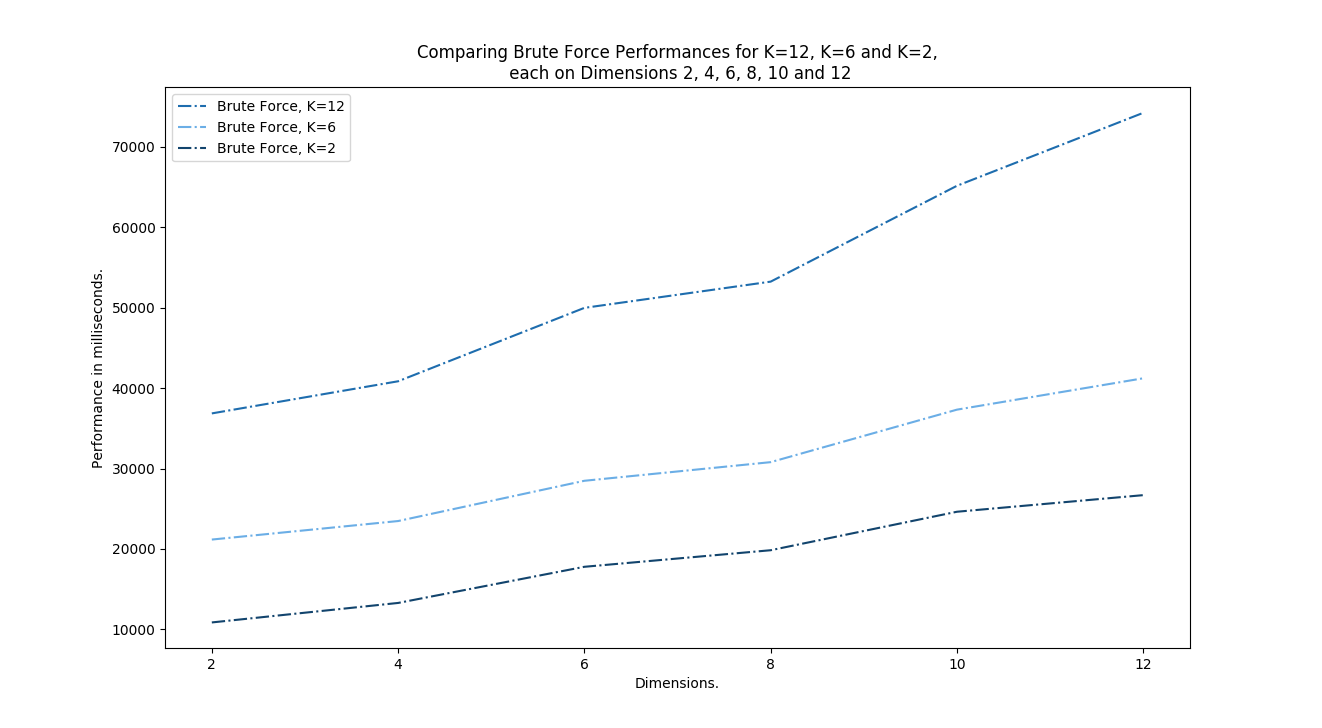
\includegraphics[width=1.1\textwidth]{pics/plot-figs/brute-k2k6k12.png}
\caption{Performance comparison of brute force, with K=12, K=6 and K=2, on datasets of sizes 1048576.}
\label{fig:b6}
\end{figure}


\begin{figure}[H]
\centering
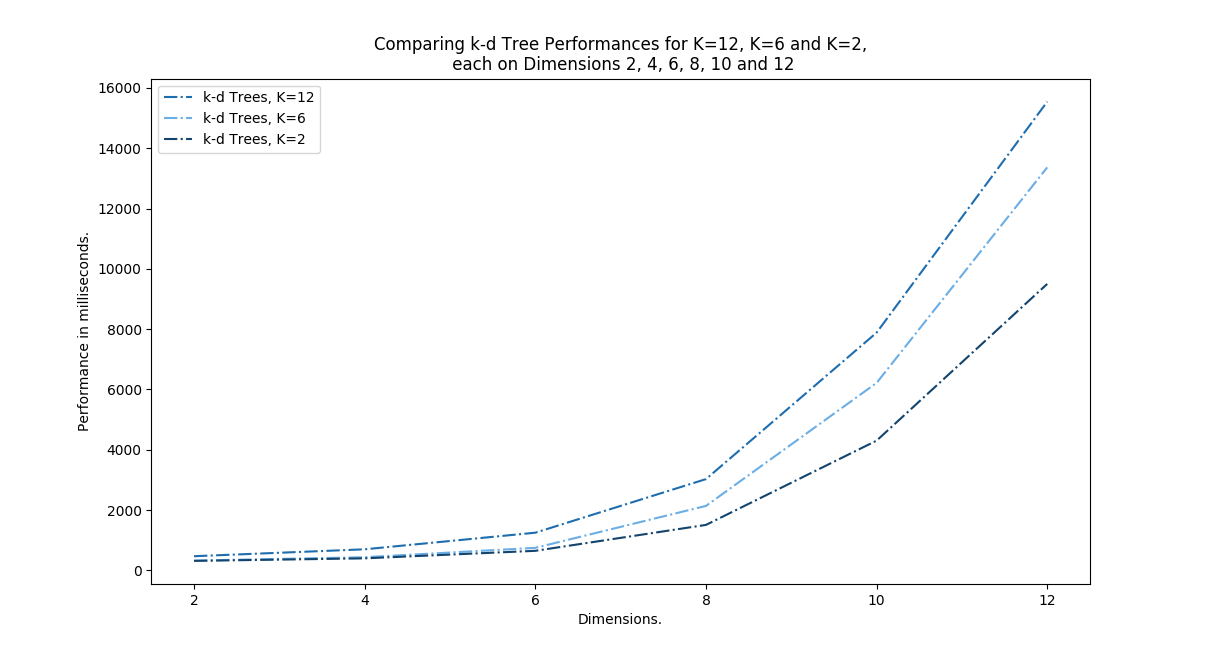
\includegraphics[width=1.1\textwidth]{pics/plot-figs/kdtree-k2k6k12.png}
\caption{Performance comparison of k-d tree, with K=12, K=6 and K=2, on datasets of sizes 1048576.}
\label{fig:b7}
\end{figure}




% The height of the tree, which dictates the number of points per leaf (?)  you need to say something about it, such as that you have run ample experiments that would take too much space to present and they indicate it is about 256 points per leaf

% Get a smallish starting point like m=100000 and then increase 400000 , 800000, 1.2mil, 1.6 mil, 2mil, 4mil, ... until it still takes reasonable time to compute.

% With high dimensionality, for large k you will wait for ages because it’s going to visit all leaves, so maybe 1, 3, 5, 7, 17 (the last one will take a while)

% Maybe d=1, 4, 6, 8, 11, 16

% 			h+1
% 100000 		9		195,3125		9	131072		256
% 400000 		11		195,3125		11	524288		256
% 800000 		12		195,3125		12	1048576		256
% 1200000		13		146,484375		13	2097152		256
% 1600000		12		195,3125		12	1048576		256
% 2000000		13		244,140625		13	2097152		256
% 4000000		14		244,140625		14	4194304		256

% x / 2^8 = 256
% x / 2^9 = 256
% x / 2^10 = 256
% x / 2^11 = 256
% x / 2^12 = 256
% x / 2^13 = 256
% x / 2^14 = 256
% x / 2^15 = 256


% 9	131072
% 11	524288
% 12	1048576
% 13	2097152
% 12	1048576
% 13	2097152
% 14	4194304

% 8	65536
% 9	131072
% 10	262144
% 11	524288
% 12	1048576
% 13	2097152
% 14	4194304
% 15	8388608
% 16	16777216
% 17	33554432


% k
% 1
% 3
% 5
% 7
% 17

% d
% 1
% 4
% 6
% 8
% 11
% 16





